The purpose of this chapter is to introduce a few of the basic ideas from classical and statistical mechanics which enter into the conceptual framework of molecular simulation.
We start by describing the classical account of the microscopic state of a system, before motivating and presenting the notion of statistical ensembles, which captures the idea of the macroscopic state of a system with many unknowable microscopic degrees of freedom.
Having presented some examples, we finally describe how dynamics on the microscopic level can in principle be thought of as a means to sample from these ensembles, thus allowing the measurement of macroscopic properties from the numerical simulation of the microscopic dynamics.

\section{The microscopic description of atomic systems}
Molecular dynamics, and computational statistical physics at large, aim at simulating on the computer the behavior of physical systems.
The hope is that one can infer quantities and properties of real-life interest from observing the results of numerical simulations, which may be relevant to understanding material properties of many-particle systems, or the nature of interactions in complex systems such as those found in biology.
Computational simulations can thus act as surrogate experiments in cases where experimental setups are hard to achieve, or measurements are impossible.
They can also be seen as surrogate tests of theoretical models, as they allow to test the validity of a mathematical description by comparing numerical predictions to experimental data. Molecular dynamics, in particular, is concerned with simulating atomic systems, most often (and as we shall systematically do) using a classical description.

\subsection{Classical phase space}

We consider a system of $N$ particles evolving in $d$-dimensional space.
The classical description contends that the \textit{state} of a system is the datum of the positions and momenta of every particle in the system.
We can interpret this as the statement that, given full knowledge of the positions and momenta at some initial time, and of the forces at play, one can deduce exactly the positions and momenta at any future time.
It is often the case in computer simulations that we consider positions which are restricted to a bounded domain by the use of periodic boundary conditions. To that effect, let
$$ \mathcal D = (L\mathbb T)^{dN} \text{or } \R^{dN}, $$
where $\mathbb T$ is the one-dimensional torus. We call $\mathcal D$ the configuration space.

\begin{definition}[Phase space]

    We describe the positions and momenta of the atoms as vectors
    $$ q=(q_{1,1},\dots,q_{1,d},\dots ,q_{N,1},\dots,q_{N,d})^\intercal \in \mathcal D,$$
    $$ p=(p_{1,1},\dots,p_{1,d},\dots ,p_{N,1},\dots,p_{N,d})^\intercal \in \R^{dN},$$
    where $q_i \defeq (q_{i,1},\dots, q_{i,d})^\intercal$ is the position vector of the $i$-th particle, and similarly for $p$. Let

    $$\mathcal E \defeq \mathcal D \times \R^{dN}.$$
\end{definition}

In this framework, the time evolution of a system can be captured by trajectories
$$(q_t,p_t)_{t\geq 0} \subset \mathcal E$$
through phase space.
It is not clear \textit{a priori} why we should choose momenta to describe the kinetic quality of the system, rather than velocities, although this is fully justified after the fact because it makes many mathematical properties simpler to state (see for example Proposition \ref{prop:hamiltonian_properties}). However, it is of no importance since we can change from one description to the other via the relation
$$v=M^{-1}p,$$
where $M\in \R^{dN \times dN}$ is a diagonal matrix recording the masses of each particle ($d$ times per particle), and $v$ is the velocity vector.
Equipped with this microscopic description, we can now describe the macroscopic state of a system, which we understand as the magnitude of certain observed quantities,
in terms of its underlying microscopic configuration.

\subsection{From microscopic states to macroscopic quantities}
The way to relate a macroscopic quantity to a microscopic state is through the general notion of an observable, which is simply a function
\[\varphi : \mathcal E \to \R \]
mapping a microscopic state to a quantity. Of course, the challenge is to define observables which are relevant in explaining pertinent macroscopic behavior.
We will not be going into the details of how formulas for these observables can be obtained, since this is a substantial part of classical mechanics. 
We refer the interested reader to \cite[Section 5.7]{T10} for an example of such a derivation in the case of pressure, while we simply state some of the observables we will be interested in.
Of utmost importance, we define the Hamiltonian, which corresponds to the total energy of the system:
\begin{equation}
    \label{eq:hamiltonian}
    H(q,p)=\frac12 p^\intercal M^{-1}p + V(q).
\end{equation}
It is the sum of two terms, the kinetic energy on the left, and the potential energy on the right, which also define respective observables of interest in their own right.
As we shall see, the Hamiltonian encodes the microscopic dynamics of the system. 
Let us note that although we restrict our discussion to real-valued observables, we can of course consider vector-valued observables, such as the force $\nabla V$.
The kinetic temperature is defined by the following expression:
$$T_\kappa (q,p)= \frac{2}{k_BdN}E_\kappa(q,p).$$
It is, up to a conversion factor of Boltzmann's constant, twice the kinetic energy per degree of freedom.
The instantaneous isotropic pressure is defined by
$$P(q,p)=\frac{1}{|\mathcal D|}\left( Nk_B T_{\kappa} -\frac1d\sum_{i=1}^N q_i^\intercal\nabla_{q_i}V(q)\right).$$
Neglecting the right-hand side gives the famous ideal gas law, $PV=Nk_BT$, which is a good approximation at low densities. The right hand side, otherwise known as the virial, appears to be problematic since the $q_i$ are not periodic functions of $q$, which would suggest $P$ is not a well-defined observable on $\mathcal D$.
However, in the case of a periodic pair interaction of the form \eqref{eq:lennard_jones}, we can use symmetry arising from Newton's third law to arrive at the following expression:
\begin{equation}\label{eq:pressure}P(q,p)=\frac1{d|\mathcal D|}\left( \sum_{i=1}^N \frac{|p_i|^2}{m_i}-\sum_{1\leq i < j\leq N}|q_i-q_j|v'(|q_i-q_j|)\right),\end{equation}


At this point, we are faced with an apparent paradox: for a system that does not display macroscopic evolution, quantities such as the energy and pressure appear constant, while the microscopic description suggest they should evolve as a function of the underlying microscopic dynamics.
A possible solution to this paradox is to move to a probabilistic description. This is the path chosen by statistical mechanics, which we now turn to by introducing the notion of a thermodynamic ensemble.

\section{Thermodynamic ensembles}
The microscopic description is interesting from a theoretical standpoint, but it fails to be relevant when attempting to describe the behavior of atomic systems with a macroscopic number of particles, of the order of Avogadro's number ($6.02 \times 10^{23} $).
Besides the technical impossibility of measuring to a high accuracy the configuration of such systems, and that of recording the information required to track it (coincidentally, the total amount of digitally stored information on Earth is estimated to be $10^{23}$ bytes as of 2022), it is also the case that knowledge of a system at this level of detail is unnecessary to describe the quantities which are relevant to our macroscopic experience.
In the instance of a gas at thermal equilibrium, examples of relevant quantities are total energy, pressure, temperature, density, which, while of course resulting from the internal state of the system, are independent of the minutiae of individual atomic motions: loosely speaking, one may describe the macroscopic state of a system by only a handful of macroscopic variables, loosing track of the myriad of microscopic degrees of freedom.
In fact, since real-valued observables map a high dimensional space to a one dimensional space, we can expect that for a given set of macroscopic conditions, there will in general be many microscopic states compatible with these conditions.
This motivates, from a purely rational point of view, passing to a statistical description: we define the macroscopic state of the system as an \textit{ensemble} of microscopic conditions compatible with the observed macroscopic constraints.
In full generality, we may further distinguish microscopic states by the likelihood they underlie the macroscopic state: this amounts to defining a probability distribution over the ensemble, or in more mathematical terms, to the data of a probability measure $\mu$ on phase space.
The macroscopic value of an observable $\varphi$ can now be interpreted as an average over the ensemble,

\begin{equation}
    \label{eq:ensemble_average}
    \E_\mu[\varphi]=\int_{\mathcal E} \varphi(q,p)\,\mu(\dif q,\dif p).
\end{equation}
This, of course, does not tell us \textit{how} we should choose such a probability measure.
However, it seems reasonable to choose, out of all probability measures which are compatible with the macroscopic constraints,
 that which contains the least information about the microscopic state, or in other words that which makes the least assumptions about it.
The mathematical translation of this idea is given by the principle of maximal entropy. Out of all probability distributions $\rho$, which for convenience we identify with smooth densities on $\mathcal E$, and which are consistent with the macroscopic constraints,
we may define the statistical ensemble as the one which maximizes the statistical entropy
\begin{equation}
    \label{eq:entropy}
    \mathfrak S(\rho)=-\int_{\mathcal E} \rho(x)\ln(\rho(x))\dx.
\end{equation}

We will be considering two examples of thermodynamic ensembles.
\subsection{Microcanonical ensemble}
    The microcanonical ensemble is the suitable model for an isolated system in thermodynamic equilibrium, evolving according to Hamiltonian dynamics. The number of particles $N$, the volume $V=L^3$, and the energy $E$ are fixed. We will alternatively refer to the microcanonical ensemble as the NVE ensemble.
     Because the constant energy condition constrains the compatible microstates to level sets of $H$, which in general will be Lebesgue-negligible subsets of $\mathcal E$, some care must be taken in defining the microcanonical measure, since one cannot express the macroscopic constraints by a family of probability densities.
      However, under suitable assumptions on $V$, one can define the microcanonical measure as a weak limit of uniform distributions over level \textquote{shells} of $H$:
    $$\int_\mathcal{E} \varphi\, \mathrm{d}\mu_{\mathrm{mc,E}} \defeq \underset{\varepsilon \to 0}{\mathrm{lim}}\, \frac{1}{|S(E,\varepsilon)|}\int_{S(E,\varepsilon)} \varphi(q,p) \mathrm{d} q \mathrm{d} p,$$
    where 
    $$S(E,\varepsilon) = \{ (q,p) \in \mathcal E |\ H(q,p) \in [E-\varepsilon,E+\varepsilon]\}.$$
    This is consistent with the fact that, for a set $A$ with finite Lebesgue measure, the probability distribution on $A$ which maximizes the entropy is the uniform distribution on $A$. 
    Alternatively, $\mu_{\mathrm{mc,E}}$ is uniquely defined by the relation
    \[\frac{1}{Z_\mathrm{E}}\int_{\mathcal E}g(H(q,p))f(q,p)\,\mathrm{d}q\mathrm{d}p=\int_{\R}g(E)\int_{\mathcal E} f(q,p)\,\mu_{\mathrm{mc,E}}(\mathrm{d} q,\mathrm{d}p)\,\dif E,\]
    for all test functions $g:\,\R\to \R$ and $f:\,\mathcal E\to \R$, and where $Z_{\mathrm{E}}$ is a normalization constant ensuring that $\mu_{\mathrm{mc,E}}(\mathcal E)=1$.
    It is possible, using the coarea formula, to derive an explicit formula for $\mu_{\mathrm{mc,E}}$, namely,

    \begin{equation}
        \label{eq:microcanonical_measure}
        \mu_{\mathrm{mc,E}}(\dif q,\dif p)=\frac 1{Z_{\mathrm{E}}}\frac{\sigma_{E}(\dif q,\dif p)}{|\nabla H(q,p)|},
    \end{equation}
    where $\sigma_{E}$ is the surface measure induced by the Lebesgue measure on the constant energy manifold
    \begin{equation}
        \label{eq:constant_energy_manifold}
        S(E) = \{ (q,p) \in \mathcal E |\ H(q,p) = E\}.\end{equation}


\subsection{Canonical ensemble}\label{par:canonical ensemble}
    Isolated systems in thermal equilibrium are not typically those that we encounter in experiments. Instead, it is more common to observe systems which are in thermal equilibrium with respect to their environment, an ambient \textit{heat bath} at a fixed temperature.
    The total energy of such systems is not fixed: small fluctuations can occur as energy is exchanged back and forth between the heat bath and the system. However, the average energy $\bar E$ is fixed. 
    This is the macroscopic constraint that defines the canonical ensemble. For fixed values $N,V,\bar E$, define the density of the the canonical measure as the maximizer:

    $$ \underset{\rho \in \mathcal A}{\mathrm{argmax}}\ \mathfrak S(\rho)$$
    where $\mathcal A$ is the set of admissible densities
    $$\mathcal A=\left\{ \rho: \mathcal E \to \R_+ \middle|\ \int_{\mathcal E} \rho =1, \int_{\mathcal E} H(q,p)\rho(q,p)\,\mathrm{d} q \,\mathrm{d} p=E \right\}.$$

    Solving the Euler-Lagrange equation associated with this constrained optimization problem yields that the only admissible solution can be written under the form:

    \begin{equation}\label{eq:canonical_measure}\mu(q,p) \defeq \frac 1{Z} \e^{-\beta H(q,p)}.\end{equation}
    Furthermore, one can show that $\mu$ is indeed the unique maximizer.
    Here, $-\beta$ and $1+\ln Z$ are the Lagrange multipliers associated respectively with the energy constraint and the normalization constraint. Thus
    $$Z=\int_{\mathcal E} \e^{-\beta H(q,p)}\,\mathrm{d} q\,\mathrm{d} p$$
    is a normalization constant called the partition function, and $\beta$ is a tuning parameter related to the value of $\bar E$. The physical interpretation of $\beta$ is that of an inverse temperature,

    $$ \beta = \frac 1{k_B T},$$
    where $k_B=1.38 \times 10 ^{-23} \mathrm{J\cdot K^{-1}}$ is Boltzmann's constant. For obvious reasons, we prefer to refer to the canonical ensemble as the NVT ensemble, rather than the NV$\bar {\text E}$.
    Besides, it can easily be shown that the canonical average of the kinetic temperature is equal to $T$, which justifies the terminology.

\begin{remark}[Other ensembles]
    One could of course go further and remark that when observing a fixed volume of unconfined gas in thermal equilibrium, the total number of particles $N$ is not fixed.
    Rather, this fluctuates as particles are constantly exchanged with an ambient particle reservoir.
    Instead, the average number of particles $\bar N$ is fixed.
    The resulting ensemble is called the grand canonical or $\mu$VT ensemble.
    This, and many other constructions are possible, but we will restrict our attention to the NVE and NVT cases. 
\end{remark}

\begin{remark}[Independence of canonical momenta and configurations]
We can make an observation on $\mu$ using the fact that the Hamiltonian \ref{eq:hamiltonian} is separable: it is the sum of a kinetic term involving $p$ and a configurational term involving $q$. Thus we can write
$$\e^{-\beta H(q,p)}=\e^{-\frac\beta 2p^\intercal M^{-1}p}\e^{-\beta V(q)},$$
which implies that the canonical measure $\mu$ is of tensor form: 
\begin{equation}\label{eq:tensor_form}\mu = \kappa \otimes \nu, \end{equation}
where $\kappa$ is a probability measure on $\R^{dN}$ has a density proportional to $\e^{-\frac\beta 2p^\intercal M^{-1}p}$ and $\nu$ has a density proportional to $\e^{-\beta V(q)}$ on $\mathcal D$.
Recognizing a multivariate Gaussian density, we can further write, abusing the notations $\kappa$ and $\nu$ to denote both the laws and their densities,
\begin{equation}
    \label{eq:kappa_marginal}
    \kappa(p)=\det(\frac{M}{2\pi\beta})^{\frac 12}\e^{-\frac\beta2p^\intercal M^{-1}p},
\end{equation}

\begin{equation}
    \label{eq:nu_marginal}
    \nu(q)=\frac1{Z_\nu}\e^{-\beta V(q)},
\end{equation}
with $$ Z_\nu= Z\det(\frac{M}{2\pi\beta})^{\frac 12}.$$
This implies in particular that the marginal distribution in $p$ of the canonical measure can be sampled easily, using standard algorithms for generating i.i.d. Gaussian variables, such as the Box-Muller method.
\end{remark}
The difficult part is thus to sample from $\nu$, as it is generally a complex and high-dimensional probability measure. 
The strategy we will use, whatever the ensemble $\widetilde{\mu}$, is to define a (possibly stochastic) dynamical system whose evolution leaves $\widetilde{\mu}$ invariant.

\section{Microscopic dynamics}
In our sense, the most important dynamics is the reference dynamics prescribed by the laws of Newtonian mechanics.
Recalling the potential $V$ in \eqref{eq:hamiltonian}, its gradient with respect to $q_i$
$$ \nabla_{q_i} V \defeq (\partial_{q_{i,d}},\dots , \partial_{q_{i,d}})^\intercal $$
gives minus the force vector acting on the $i$-th particle. In our case we will always take the potential to be independent of the momentum, so that we can think of $V$ as having domain $\mathcal D$. In the case where $\cD = (L\mathbb T)^{dN}$, it will be convenient to think of $V$ as a function from $\R^{dN}$ to $\R$ which is $C^1$ and $L$-periodic in each direction.
As it encodes the dynamics of the system, the potential $V$ is of paramount importance. Indeed, the time evolution of the system is then described by Newton's second law:

\[M\ddot{q}=-\nabla V(q).\]

It will be convenient for our analysis to use of reformulation of Newton's equations, based on the Hamiltonian of a system.
Using the Hamiltonian \eqref{eq:hamiltonian}, we can rewrite the classical equations of motion as

\begin{equation}
\label{eq:hamiltonian_dynamics}
\begin{cases}
    \mathrm{d} q_t=M^{-1}p_t\dt=\nabla_p H(q_t,p_t)\dt\\
    \mathrm{d} p_t=-\nabla V(q_t)\dt=-\nabla_q H(q_t,p_t)\dt
\end{cases},
\end{equation}

The potential energy is the most important part of the microscopic description, and accordingly, the first and foremost problem in establishing a physical model of this kind is to determine find a potential whose corresponding dynamics faithfully reproduce a given desirable macroscopic behavior.
The choice of a classical description automatically implies a degree of approximation, since behavior arising from the laws of quantum mechanics, which may be relevant at a microscopic level, have to be reproduced in a Newtonian framework.
 Furthermore, if the aim is to simulate such systems numerically, computational constraints imply that some compromise has to be reached between theoretical accuracy and computational cost. 
 If, for small systems, it may be possible to simulate all atomic interactions, for larger or more complex systems, it is often only feasible to use potential functions which are both cheap from a computational point of view and empirically shown to be accurate enough for the purpose of a simulation.

 Our main numerical example will be the system given by the following empirical potential, and which is often used to describe the microscopic behavior of chemically inert fluids, such as Argon.

 \begin{example}[The Lennard--Jones fluid]
    We fix $L>0$ and $d=3$. The Lennard-Jones fluid is the classical system given by the pair-interaction potential

    \begin{equation}
        \label{eq:lennard_jones}
        V_{\mathrm{LJ}}(q)=\sum_{1\leq i < j \leq N} v(|q_i-q_j|),        
    \end{equation}
    where $v$ is the radial function

    $$v(r)=4\varepsilon \left( \left( \frac{\sigma}{r}\right)^{12}-\left(\frac{\sigma}{r} \right)^6\right).$$
    The reference energy $\varepsilon$ and length $\sigma$ are shape parameters which respectively control the depth of the potential well and the equilibrium distance $2^{1/6}\sigma$.
    As seen on Figure \ref{fig:lennard_jones}, the potential combines two effects. At small interparticular distances, the dominant term is in $r^{-12}$, which translates into a strongly repulsive force between close pairs of particles, and makes individual particles essentially impenetrable.
    At long range, the dominant term is in $-r^6$, which translates into a weakly attractive force between distant particles. Contrary to the repulsive term, which is empirical, this scaling has a theoretical origin in the Van der Waals forces.
    From a computational standpoint, the fact that $v$ is an even function of $r$ allows one to compute the normalized force while sparing the expense of computing a square root, while the identity $r^{12}=(r^6)^2$ allows further economy.
    The shape parameters $\sigma$ and $\varepsilon$ must be chosen empirically to describe the behavior of a particular atomic species.
 \end{example}

 \begin{figure}[htbp]
    \begin{center}
      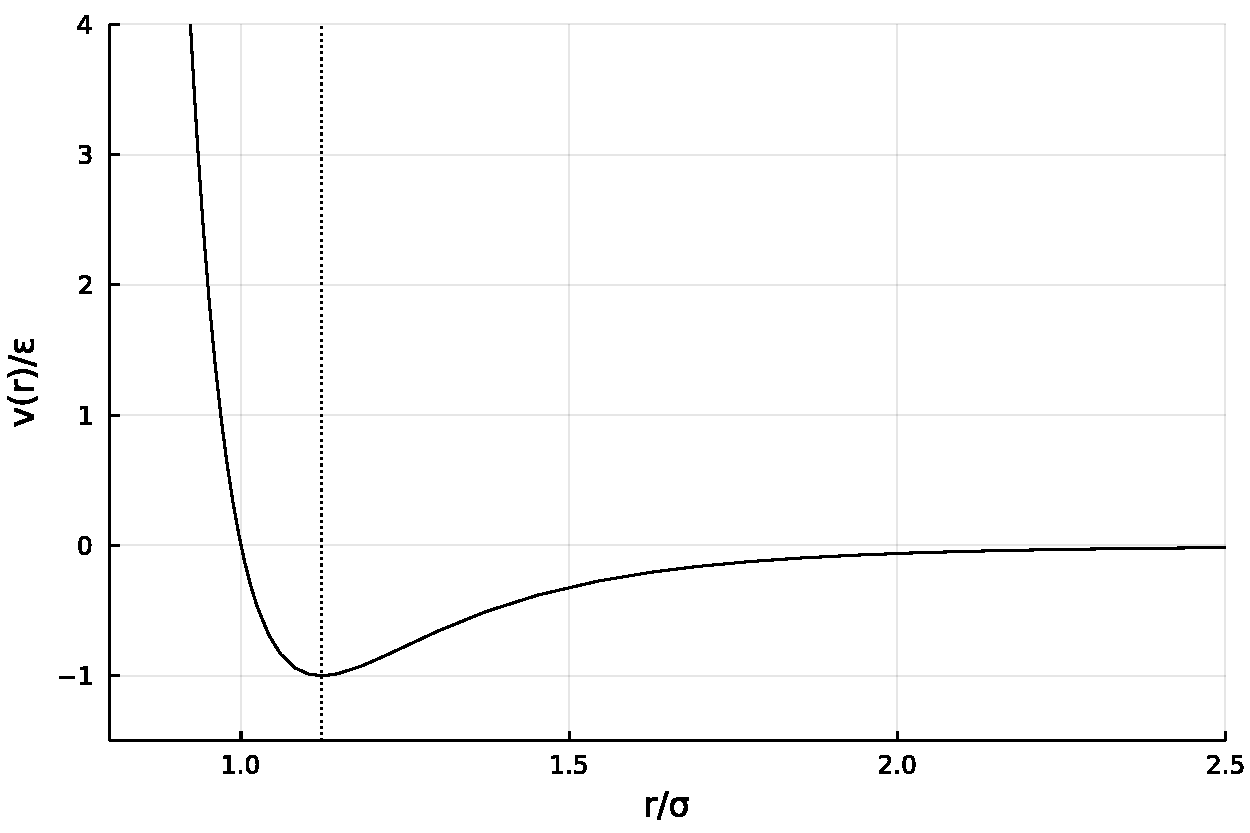
\includegraphics[width=0.7\linewidth]{figures/chapter1/lennard_jones.pdf}
      \caption{ \label{fig:lennard_jones}
        The pair potential $v$, with distances and energy given in reduced units. The equilibrium interparticular distance is indicated by the vertical dotted line.
      }
    \end{center}
  \end{figure}

\subsection{Reduced units}
It is convenient, given an atomic system, to describe quantities therein within a system of units in which they are of order one. This has several advantages. 
Firstly, like any reasonable system of units, reduced units make quantities easier and more intuitive to reason about.
Secondly, from the computational point of view, numerical artifacts due to loss of precision at very large or very small scales and overflow errors can be avoided more often.
Thirdly, they may help transfer knowledge about one system to another. 
For instance, in the Lennard-Jones system, expressing a quantity in reduced units,
and knowing the dependency of these units on the parameters $(\varepsilon,\sigma,M)$ of the system, one can infer properties about a system with parameters $(\tilde\varepsilon,\tilde\sigma,\tilde M)$ by applying the inverse transformation, thus effectively yielding equivalence of different systems under different conditions, and sparing the cost of running redundant simulations.

We describe a general procedure to construct a set of reduced units. Our choice, although not necessarily unique, is quite natural, especially when dealing with the Lennard--Jones system.
Let us fix a reference mass $m_*$, a reference energy $\varepsilon_*$ and a reference length $\sigma _*$. Then various reference quantities can be derived by natural conversions and dimensional analysis:
\begin{align*}&t_*=\sqrt{\sigma_*^2m_*\varepsilon_*^{-1}},\tag{time}\\
    &T_*=\varepsilon_*k_B^{-1},\tag{temperature}\\
    &v_*=\sigma_*t_*^{-1},\tag{velocity}\\
    &V_*=\sigma_*^3,\tag{volume}\\
    &A_*=\sigma_*^2,\tag{area}\\
    &\rho_*=V_*^{-1},\tag{density}\\
    &F_*=m_*\sigma_*t_*^{-2},\tag{force}\\
    &P_*=F_*A_*^{-1},\tag{pressure}
\end{align*}
and one can of course go on. The point is that if $X$ is a quantity, one can obtain its reduced value $X_{\mathrm{red}}$ by dividing $X$ by the reference quantity $X_*$ which is dimensionally compatible with $X$, and which can be derived as above.
For instance, given a pressure $P$, we obtain
$$P_{\mathrm{red}}= P\sigma_*^3\varepsilon_*^{-1}.$$
Note this is an adimensional quantity. Note, also that, due to the definition of the reference temperature $T_*$ relative to the reference energy $\varepsilon_*$, energies are now commensurate to temperatures.
The Boltzmann factor, which is the conversion factor between units of temperature and units of energy simplifies when expressed in reduced units, a fact we can capture with the maxim ${k_B}*=1$. This simplifies many formulae.

For a monatomic Lennard--Jones system, a natural choice for $m_*$ is the atomic mass of the considered species. We also take $\varepsilon_*=\varepsilon$ and $\sigma_*=\sigma$ (although the equilibrium length $\sigma=2^{1/6}\sigma$ is another possible choice). In the case of Argon, we use the following values:
$$m_*=6.634 \times 10 ^{-26}\, \text{kg},\ \sigma_*=3.405 \times 10^{-10}\, \text{m},\ \varepsilon_*=1.66 \times 10^{-21}\, \text{J}.$$
Unless explicitly specified, all numerical results will be in this system of reduced units.

Once a dynamic has been prescribed, and an observable of interest as been fixed, we can describe our strategy to sample from a thermodynamic ensemble.

\subsection{Ergodic averages}
We define a process $(q_t,p_t)_{t\geq 0}$ on $\mathcal E$, either deterministic or stochastic, which is invariant for the target measure $\widetilde{\mu}$, in the following sense:
for all $t\geq 0$ and all bounded measurable observable $\varphi$, we require
\begin{equation}
    \label{eq:invariant_measure}
    \int_{\mathcal E}\E^{(q,p)}\left[ \varphi(q_t,p_t)\right]\,\widetilde{\mu}(\mathrm{d}q,\mathrm{d}p)=\int_{\mathcal E}\varphi(q,p)\,\widetilde{\mu}(\mathrm{d}q,\mathrm{d}p),
\end{equation}
where the superscript in the expectation denotes that the process has value $(q,p)$ at $t=0$, and the expectation is over realizations of $(q_t,p_t)$. In other words, this is a process which, given that its initial condition is distributed according to $\widetilde{\mu}$, remains distributed according to $\widetilde{\mu}$ at any later time. It is then natural to consider average values of $\varphi$ over the trajectories:
\begin{equation}
\label{eq:ergodic_averages}
 \widehat{\varphi}_T \defeq \frac{1}{T}\int_{0}^T \varphi(q_t,p_t)\,dt,
\end{equation}
which we may hope will converge to the target ensemble average \eqref{eq:ensemble_average}. 
The convergence of ergodic averages to the ensemble average can be shown not to hold in generality, and is something which must be proven on a case by case basis, though general criteria can be derived, see for instance \cite{K87}.
If the underlying dynamic is stochastic, then the variance of the random variables \eqref{eq:ergodic_averages} becomes an issue, which one must control by ensuring that time averages are taken over long enough trajectories. 
Furthermore, since the true invariant dynamics is in general in continuous time, one must generally devise discrete-in-time approximations to the true trajectories.
However, empirical practice shows that ergodic averages obtained from computer simulations, even for a modest number of atoms, agrees very well with experimental data for certain types of systems, and even in the absence of theoretical guarantees.